
    \documentclass[12pt]{report}  % Using 'report' class to avoid blank pages between chapters
    \usepackage{setspace}
    \usepackage{titlesec}
    \usepackage{graphicx}
    \usepackage{url}
    \titleformat{\chapter}[display]
      {\normalfont\huge\bfseries}{\chaptername\ \thechapter}{20pt}{\Huge}
    \usepackage{fancyhdr}
    \pagestyle{fancy}
    \fancyhf{}
    \rhead{\thepage}
    \begin{document}
    \onehalfspacing
    \pagenumbering{gobble} % Suppress page numbers until Chapter 1
    \begin{center}\n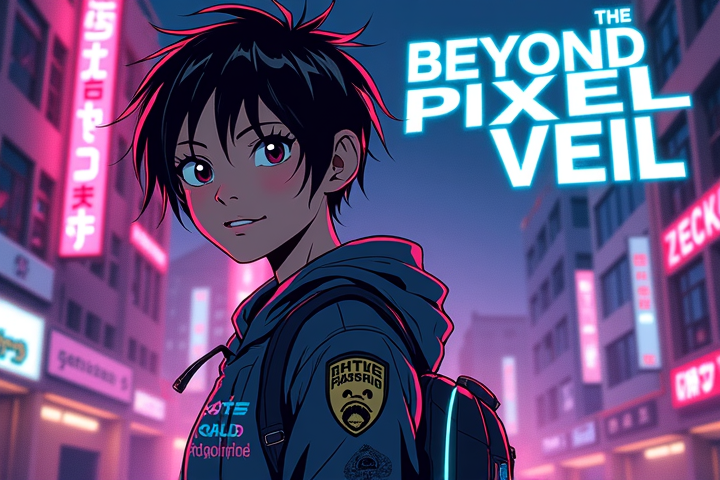
\includegraphics[width=0.8\textwidth]{stories/my_story/step_6/scenes/title.png}
\vspace{1cm}

    {\Huge \textbf{Beyond the Pixel Veil}} \\[2cm]
    \end{center}
    
    \newpage
    \pagenumbering{arabic} % Start page numbering
    \chapter*{Chapter 1: The Underdog's Rise}
\addcontentsline{toc}{chapter}{Chapter 1: The Underdog's Rise}
\textit{Meera participates in a high-stakes Eon gaming tournament, showcasing her extraordinary skills.}

\begin{center}
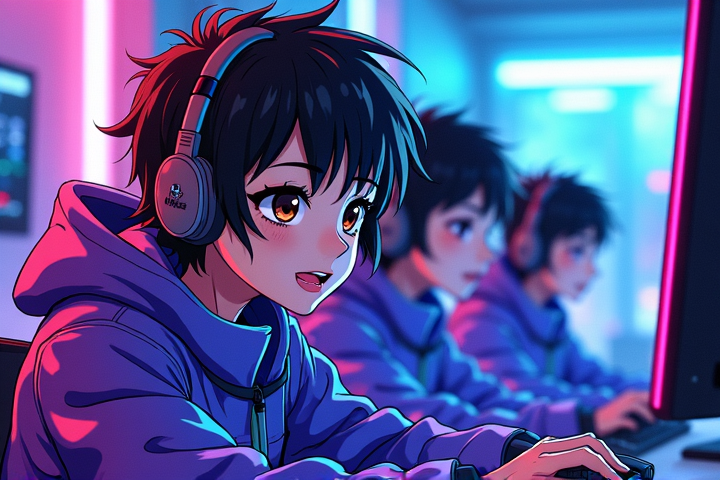
\includegraphics[width=0.8\textwidth]{stories/my_story/step_6/scenes/gaming_tournament.live.png}
\end{center}

The air was electric with anticipation as Meera 'Midnight' Singh stepped
onto the vibrant, neon-lit stage of New Mumbai's Cyber Arena. The
crowd's deafening roar enveloped her, a cacophony of cheers and chants
that threatened to consume her entire being. With a deep breath, she
slipped on her trusty headset, the familiar weight a comforting reminder
of the battles she was about to face.

As she gazed out into the sea of expectant faces, Meera's thoughts
drifted back to the countless hours spent honing her craft in cramped,
dimly lit internet cafes. The underdog from the outskirts of New Mumbai
had finally made it to the big leagues - the Eon Gaming Tournament's
grand finale. Her team, 'Midnight's Marauders,' was set to take on the
reigning champions, 'Specter's Squad,' led by the charismatic Jax
'Specter' Lee.

Meera's eyes locked onto her teammates, each one a vital cog in their
well-oiled machine. There was Rohan 'Brawler' Jensen, their tanky
powerhouse; Leela 'Lumina' Rao, the team's brilliant strategist; and
lastly, Meera herself - 'Midnight,' the enigmatic, quick-witted
assassin. Together, they had defied all odds to reach this moment.

The tournament's AI, EVE, boomed to life, her melodic voice echoing
through the arena. "Welcome, gamers and spectators, to the Eon Gaming
Tournament's grand finale! On my mark, the battle for supremacy will
commence. Three... two... one... \textbf{Eon Initiated!}"

The arena's massive screens flickered to life, displaying the game
world: a dystopian metropolis known as 'Neo-Eden.' Meera's team
materialized within the virtual realm, their avatars assuming their
designated roles. The opposition, Specter's Squad, emerged at the
opposite end of the map, their confident smirks visible even through the
digital facades.

The match began with a flurry of activity - spells were cast, bullets
flew, and the two teams clashed in a spectacular display of light and
sound. Meera's fingers danced across her controller, each press and
swipe executed with precision. Her assassin avatar weaved between
skyscrapers, exploiting the shadows to pick off stray opponents.

As the battle raged on, an unusual sensation began to build within Meera
- a tingling, electric feeling that seemed to emanate from the very core
of the game itself. It was as if Eon's underlying code was resonating
with her, attuning itself to her every move. The experience was both
exhilarating and unsettling, like being on the cusp of unlocking a
hidden potential.

With the clock ticking down, Midnight's Marauders found themselves on
the back foot, Specter's Squad having gained a slender lead. Meera's
team huddled around Leela, who rapidly outlined a daring plan to turn
the tide. The strategy relied heavily on Meera's unorthodox skills -
could she pull off the impossible?

The crowd held its collective breath as Meera's avatar broke away from
the group, embarking on a perilous solo mission. She sprinted across
Neo-Eden's rooftops, the electric sensation surging to a fever pitch.
Time seemed to slow, and for an instant, Meera felt an unshakeable
connection to the digital realm - as if she could manipulate the very
fabric of Eon.

In a heart-stopping, action-packed sequence, Meera's avatar executed a
series of death-defying leaps, closing in on Specter's Squad's
vulnerable base. The opposition scrambled to respond, but Meera was an
unstoppable force, her movements guided by the strange, symbiotic link
with the game.

The arena erupted into pandemonium as Midnight's Marauders emerged
victorious, having overturned the deficit in a stunning upset. Meera's
teammates lifted her onto their shoulders, basking in the adoration of
the crowd. As she gazed out at the sea of faces, now filled with a mix
of awe and curiosity, Meera couldn't shake off the feeling that
something fundamental had shifted within her - that this victory was
merely the beginning of an extraordinary journey.

As the team celebrated, Meera's thoughts drifted back to the enigmatic
sensation, now dormant but still lingering, like the promise of a
gathering storm. She smiled, unsure what the future held, but ready to
face whatever challenges lay beyond the screen.


\chapter*{Chapter 2: Awakening to Nexus}
\addcontentsline{toc}{chapter}{Chapter 2: Awakening to Nexus}
\textit{Meera discovers she can manipulate the Nexus, an alternate reality, through her gaming skills.}

\begin{center}
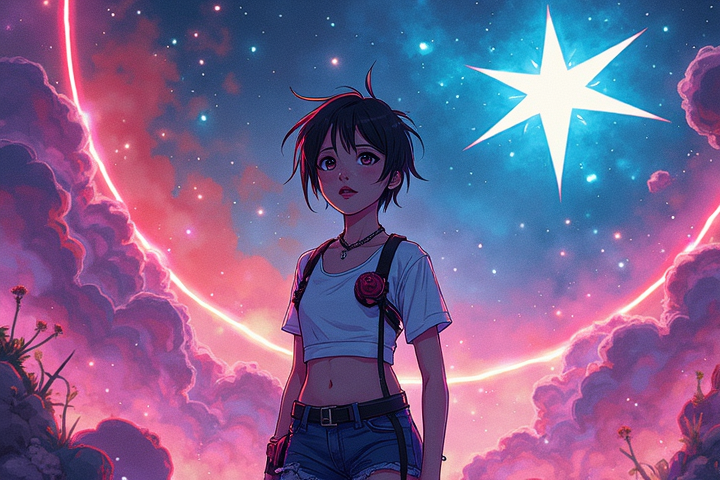
\includegraphics[width=0.8\textwidth]{stories/my_story/step_6/scenes/nexus_awakening.live.png}
\end{center}

The world around her dissolved like pixels on a fading screen. Meera's
senses, once anchored to the familiar rhythms of New Mumbai's Cyber
Arena, now drifted on an ethereal tide. The last remnants of the gaming
tournament - the cheers, the pulsating lights, and Jax's triumphant
whoop - receded into the distance, replaced by an unsettling stillness.

As she floated, weightless, Meera became aware of a gentle, luminescent
glow enveloping her. The light was soft as a summer breeze, yet it
illuminated every detail of her surroundings with eerie precision. She
found herself suspended within a boundless, star-filled expanse, the
celestial bodies twinkling like diamonds scattered across the velvet
blackness.

A presence coalesced beside her, its arrival heralded by a subtle shift
in the glow's intensity. Meera turned to face the newcomer, her heart
beating with a mix of trepidation and curiosity. The being, humanoid in
shape yet crafted from the very essence of the stars, regarded her with
an unblinking gaze.

"Greetings, Meera 'Midnight' Singh," the being said, its voice like the
harmonious resonance of a thousand glass wind chimes. "I am Astrum,
Guardian of the Nexus. Your... unique connection to our realm has been
noted."

Meera's mind struggled to keep pace with the surreal events unfolding
around her. "Nexus?" she repeated, the word feeling foreign on her lips.
"What do you mean? One minute I was gaming, and the next... this."

Astrum's luminous form undulated, as if the Guardian were nodding. "The
Nexus is an intersecting plane, a realm where the fabric of reality is
woven from the threads of human imagination and innovation. Your
exceptional skills within Eon have created a... resonance, allowing you
to transcend the boundaries between worlds."

As Astrum spoke, the starry expanse around them began to transform.
Nebulae coalesced into gleaming, iridescent architectures that defied
gravity and logic. Meera felt her perception expanding, as if her very
brain was being rewired to comprehend the impossible geometries of this
new realm.

"What do you want from me?" she asked, a sense of trepidation creeping
up her spine. The vast, uncharted expanse of the Nexus stretched out
before her like an endless, shimmering sea.

Astrum's gaze turned inward, as if consulting a deep, cosmic wisdom.
"The balance of the Nexus is precarious, Meera. A discordant force
threatens to unravel the fabric of our realm, with repercussions that
would be catastrophic for both your world and ours. We believe your
unique connection makes you an ideal... catalyst. One who can help
restore harmony to the Nexus."

The weight of Astrum's words settled upon Meera like a physical burden.
She thought of her life in New Mumbai, her friends, and her family - all
seemingly light-years away from this fantastical, star-born realm.

"What makes you think I'm the right person for this?" she asked, a hint
of skepticism creeping into her voice.

Astrum's response was immediate: "Because, Meera 'Midnight' Singh,
within the Nexus, your potential is limitless. The question is... will
you choose to embrace it?"

As the Guardian's words hung in the balance, Meera felt the first
tremors of a transformation, one that would forever alter the trajectory
of her life. The stars around her pulsed in anticipation, as if the very
fabric of reality was holding its breath, waiting for her response.


\chapter*{Chapter 3: Confronting Rivals}
\addcontentsline{toc}{chapter}{Chapter 3: Confronting Rivals}
\textit{Meera encounters Jax 'Specter' Lee, Dr. Zhang 'Zen' Wei, and Maya 'Rampart' Patel at a gaming event.}

\begin{center}
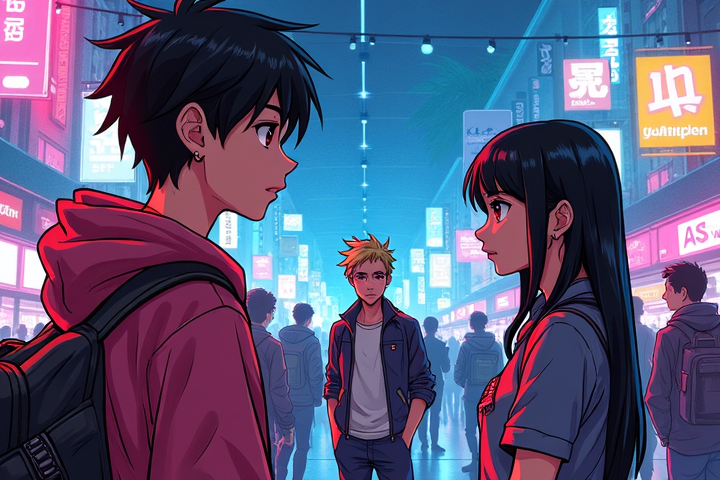
\includegraphics[width=0.8\textwidth]{stories/my_story/step_6/scenes/rival_encounter.live.png}
\end{center}

The air was electric with anticipation as Meera navigated through the
crowded Gaming Expo, her eyes scanning the sea of colorful booths and
enthusiastic attendees. The hum of lively chatter, the wail of excited
screams, and the pulsating rhythms of electronic dance music all blended
together in a cacophony that was both overwhelming and exhilarating.
Meera's heart thrummed in time with the beat, her senses heightened as
she searched for the one place she knew her rivals would be.

As she turned a corner, a sprawling banner emblazoned with "Specter's
Squad" caught her attention, accompanied by an enormous, inflated gaming
chair that seemed to glow with an otherworldly aura. Meera's gaze
narrowed; this was the spot. With a deep breath, she steeled herself for
the encounter ahead and wove through the throng of fans gathered around
the booth.

Jax "Specter" Lee, resplendent in his signature black leather jacket
adorned with neon green accents, held court before a mesmerized
audience. His quick wit and effortless charm had the crowd eating out of
the palm of his hand as he regaled them with tales of his gaming
prowess. Meera's eyes met Jax's for a fleeting instant, a spark of
mutual awareness flashing between them before he seamlessly continued
his performance.

To the side, Dr. Zhang "Zen" Wei sat engrossed in a heated game of
\emph{Eon: Reckoning}, her slender fingers flying across the controller
with a speed and precision that belied her calm demeanor. The soft glow
of the gaming station illuminated her features, casting an ethereal
light on the sharp planes of her face. Meera noticed the faintest hint
of a furrowed brow, a telltale sign that Dr. Zhang was fully invested in
the game.

Maya "Rampart" Patel, meanwhile, stood at the periphery, observing the
scene with an air of quiet intensity. Her piercing green eyes seemed to
bore into Meera as their gazes met, a flicker of curiosity dancing
across her face before she returned to surveying the crowd. The
intricate, glow-in-the-dark tattoos on her arms appeared to pulse in
rhythm with the music, adding to the enigmatic aura surrounding her.

Meera's approach did not go unnoticed for long. As she drew closer,
Jax's narrative began to wind down, and he flashed her a disarming
smile. "Well, well, well. Look what we have here. If it isn't Midnight
herself, emerging from the shadows."

The crowd, sensing a potential confrontation, began to murmur excitedly,
their attention shifting toward Meera like a tidal wave. Dr. Zhang
paused her game, her eyes locking onto Meera with interest, while Maya's
gaze never wavered, her expression unreadable.

"Jax," Meera said, her voice even, "I think we need to talk."

The smile on Jax's face grew wider as he spread his arms, encompassing
the booth. "The floor is yours, Midnight. We're all ears... and eyes, of
course." He winked at the crowd, which responded with a chorus of
laughter and applause.

Meera's cheeks flushed slightly, but she pressed on, her focus solely on
the trio before her. "I'm sure you're all aware of the recent...
developments in Nexus."

Dr. Zhang's eyebrows arched, her interest piqued. "You're referring to
the anomalies?"

Meera nodded. "Yes. I believe our unique skill sets could be crucial in
navigating these changes. I propose an alliance - temporary, if that's
what you prefer - to tackle the challenges Nexus has in store for us."

The booth fell silent, the only sound the distant thrum of the expo.
Jax, Dr. Zhang, and Maya exchanged weighted glances, their expressions a
kaleidoscope of emotions: skepticism, curiosity, and, perhaps, a hint of
intrigue.

It was Maya who broke the silence, her voice low and even. "What makes
you think we'd be interested in teaming up with you, Midnight? We're not
exactly... friends."

Meera stood tall, meeting Maya's gaze head-on. "I'm not asking for
friendship; I'm asking for cooperation. Together, we could achieve
something remarkable. And who knows?" A hint of a smile played on her
lips. "We might just learn to trust each other in the process."

As Meera's words hung in the air, Jax leaned back in his chair,
steepling his fingers together in a gesture of contemplation. Dr. Zhang
returned to her game, though her eyes darted toward Meera at intervals,
as if reassessing her. Maya, however, remained still, her gaze burning
with an intensity that made Meera's skin prickle.

The crowd, sensing the tension, began to disperse, murmuring among
themselves about the potential alliance. The expo's ambient noise slowly
reclaimed the space around the booth, a reminder that, despite the
gravity of their discussion, the world beyond this moment continued to
spin.

Jax was the first to break the silence, his voice laced with a hint of
amusement. "Well, Midnight, it seems you've certainly given us something
to think about. Why don't we discuss the details over dinner? My treat."

Dr. Zhang paused her game once more, a small, enigmatic smile playing on
her lips. "I'm in. But just for the food, and perhaps a glimpse into
your strategy, Meera."

Maya's response was the longest in coming, her eyes never leaving
Meera's face. Finally, she nodded, a curt, economical motion. "Fine. But
if this is a ploy to sabotage us, Midnight... let's just say I have
measures in place."

With that, the unlikely allies began to make their way out of the booth,
the expo's vibrant chaos swallowing them whole as they embarked on a
journey that would change the course of their lives - and the fate of
Nexus - forever.


\chapter*{Chapter 4: First Trial in Nexus}
\addcontentsline{toc}{chapter}{Chapter 4: First Trial in Nexus}
\textit{Meera and her new allies face their first challenge in the Nexus, testing their teamwork.}

\begin{center}
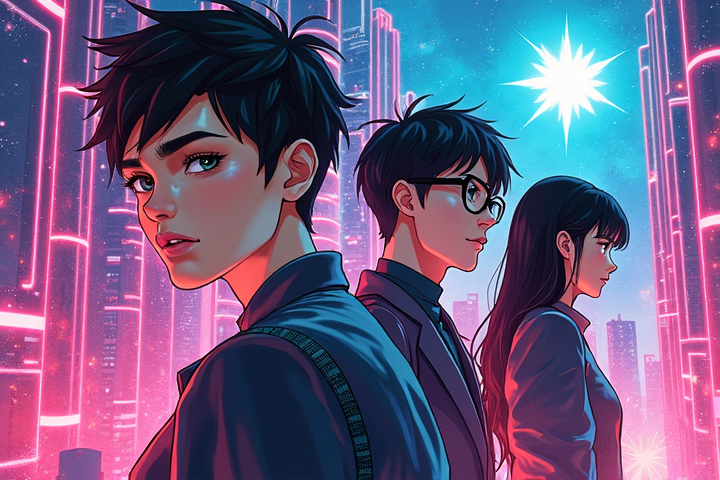
\includegraphics[width=0.8\textwidth]{stories/my_story/step_6/scenes/nexus_challenge.live.png}
\end{center}

The air was alive with an otherworldly energy as Meera stepped into the
Nexus Realm alongside her unlikely allies. The Maze of Reflections,
their first trial, stretched before them like a labyrinthine canvas of
shimmering silver and gold. Eternal dawn cast its ethereal glow upon the
landscape, imbuing every step with an aura of anticipation.

"Reflections, huh?" Jax 'Specter' Lee murmured, his eyes scanning the
ever-shifting pathways. "Sounds like a walk in the park... for
philosophers."

Dr. Zhang 'Zen' Wei's gaze remained fixed on the maze, her expression
introspective. "The Nexus Guardian warned us: our perceptions will be
challenged. We must trust not just each other, but ourselves."

Maya 'Rampart' Patel adjusted her armguards, a hint of a smile playing
on her lips. "Time to put that trust to the test. Let's move out!"

Meera took a deep breath, the weight of her responsibilities settling
more comfortably with each passing moment. She nodded, and together they
ventured into the heart of the maze.

As they navigated the twisting passages, illusions began to manifest
around them. Reflections of their deepest fears and desires coalesced
into tangible, ghostly apparitions that darted at the edges of their
vision. Meera's own reflections taunted her: visions of failure in the
gaming tournament, of losing control in the Nexus, and of the
devastating consequences on Earth.

"Focus on your surroundings, not the illusions," Dr. Zhang advised, her
voice calm and reassuring. "The maze responds to our collective
perceptions. Unity is key."

Jax snorted. "Easy for you to say, Zen. You're not the one with a
reflection that's trying to convince me I'm a has-been streamer."

Maya chuckled, her defensive stance unwavering. "Hey, Specter, your ego
can take it. We've got more pressing concerns... like that."

She gestured toward an intersection where multiple pathways converged.
Each route was guarded by a reflection of one of their allies, each
apparition embodying a conflicting aspect of their personalities.

Meera's gaze met the reflections, and she realized the true nature of
the challenge. "We need to choose which aspects of ourselves to trust...
and which to overcome."

With newfound determination, Meera led the way, selecting paths that
balanced their collective strengths and weaknesses. As they progressed,
the illusions intensified, but so did their trust in each other. Jax
began to acknowledge Maya's strategic prowess, while Dr. Zhang found
solace in Meera's instinctive leadership.

The final trial awaited them at the maze's center: a mirrored chamber
where their reflections merged into a single, unified apparition. The
specter embodied both their greatest fears and most profound
aspirations, its presence both captivating and terrifying.

"We are the sum of our parts," the apparition declared, its voice an
echo of their collective consciousness. "Trust in yourselves, and you
shall find harmony within the Nexus."

As one, Meera and her allies reached out, their hands meeting at the
heart of the illusion. The mirrored chamber shattered, releasing a
kaleidoscope of light that enveloped them.

When the radiance dissipated, they found themselves standing before the
Nexus Guardian, Astrum's luminous form aglow with approval.

"Well done, travelers," Astrum said, its voice like celestial music.
"You have passed the first trial, learning to trust not only each other,
but the depths of your own hearts. The path ahead will be fraught with
greater challenges... but together, you shall illuminate the darkness."

As they emerged from the Maze of Reflections, Meera shared a glance with
her allies, their bond forged in the heart of the Nexus. Together, they
stood ready to face whatever trials lay ahead, their trust in each other
burning brighter than any illusion.


\chapter*{Chapter 5: Aftermath on Earth}
\addcontentsline{toc}{chapter}{Chapter 5: Aftermath on Earth}
\textit{Meera witnesses the devastating effects of her Nexus actions on Earth, including loss of life.}

\begin{center}
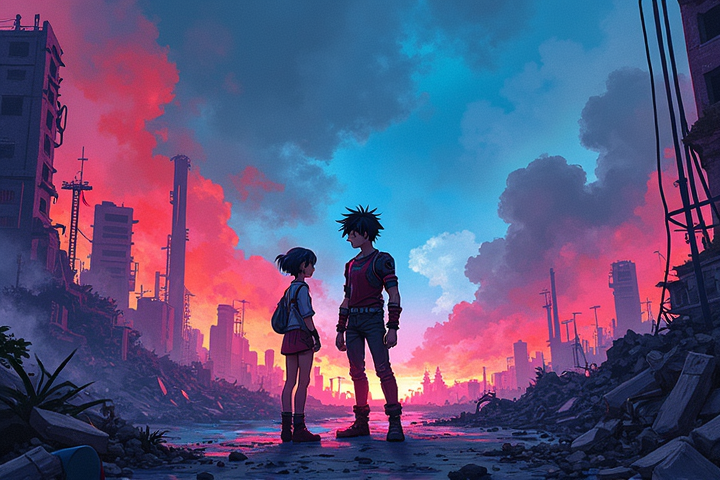
\includegraphics[width=0.8\textwidth]{stories/my_story/step_6/scenes/earth_aftermath.live.png}
\end{center}

The darkness was absolute, punctuated only by the faint hum of emergency
generators and the soft murmur of hushed conversations. Meera's eyes,
accustomed to the vibrant neon hues of New Mumbai's cityscape, struggled
to adjust to the dimly lit landscape before her. The air reeked of
smoke, ozone, and desperation.

As she stepped out of the makeshift medical tent, the chill of the night
air enveloped her, carrying with it the whispers of the devastated.
Meera's gaze wandered across the sea of makeshift shelters, the
rubble-strewn streets, and the twisted wreckage of what once were homes.
The weight of her actions in the Nexus crushed her, threatening to
consume her very being.

"Meera, we need to talk," a low, urgent voice called out from beside
her.

She turned to face Kaito 'Sparrow' Hernandez, leader of the underground
rebellion against the corporations exploiting Eon. His bright hazel
eyes, usually ablaze with determination, now seemed dulled by the
exhaustion and grief etched on his face.

"Kaito... I..." Meera's voice faltered, her throat constricting as she
struggled to find words to express the turmoil within her.

Sparrow's expression softened, and he placed a gentle hand on her
shoulder. "Not here, not now. Follow me."

He guided her through the winding paths of the disaster zone, dodging
rescue workers and volunteers as they navigated the treacherous terrain.
They eventually stopped at a small, partially intact cafe, its walls
bearing the scars of the catastrophe. Sparrow pushed open the creaky
door, and Meera followed him inside.

The cafe's interior was a stark contrast to the chaos outside. The
tables, though scarred, were clean; the chairs, albeit battered, stood
upright. A small, battery-powered lantern cast a warm glow over the
space, illuminating the faces of those gathered within. Meera recognized
some of them as members of Sparrow's rebellion.

Sparrow led her to a corner table, where a steaming cup of coffee
waited. "Drink this, you look like you could use it," he said, his voice
low and soothing.

Meera wrapped her hands around the warm cup, feeling the heat seep into
her chilled bones as she took a tentative sip. The bitter flavor helped
clear her mind, allowing her to focus on Sparrow's expectant gaze.

"What do you know about the... the incident?" Meera asked, her voice
barely above a whisper.

Sparrow's expression turned grim. "We've confirmed at least three major
corporations were involved in exploiting Eon's energy grid. Your actions
in the Nexus... they triggered a catastrophic resonance cascade,
amplifying the energy feedback into our world."

Meera felt as though she'd been punched in the gut. "How many...?"

Sparrow's eyes dropped, his voice cracking. "We've counted over five
hundred confirmed fatalities so far. Thousands more are injured or
missing. The city's infrastructure is in shambles."

The coffee cup slipped from Meera's grasp, shattering on the floor as
she buried her face in her hands. The weight of her responsibility
threatened to consume her, the screams of the victims echoing in her
mind.

Sparrow's hand found its way back to her shoulder, his grip firm but
comforting. "Meera, listen to me. This wasn't just your fault. The
corporations knew the risks; they gambled with people's lives. You were
a catalyst, but you're not the sole cause."

His words offered little solace, but Meera appreciated the attempt. She
raised her head, meeting Sparrow's gaze. "What can I do to help?"

A hint of determination crept back into his eyes. "We need to take down
the corporations responsible. We have evidence, but we require someone
with your... unique connection to the Nexus. Will you join us, Meera?
Help us bring them to justice?"

As Meera searched Sparrow's face, she knew her answer would forever
alter the course of her life. The darkness outside seemed to press in,
awaiting her response. With a deep breath, she made her decision.

"I'm in."


\chapter*{Chapter 6: Confronting the Architect}
\addcontentsline{toc}{chapter}{Chapter 6: Confronting the Architect}
\textit{Meera and her allies confront the enigmatic Architect (Erebus), seeking answers about Nexus and Eon.}

\begin{center}
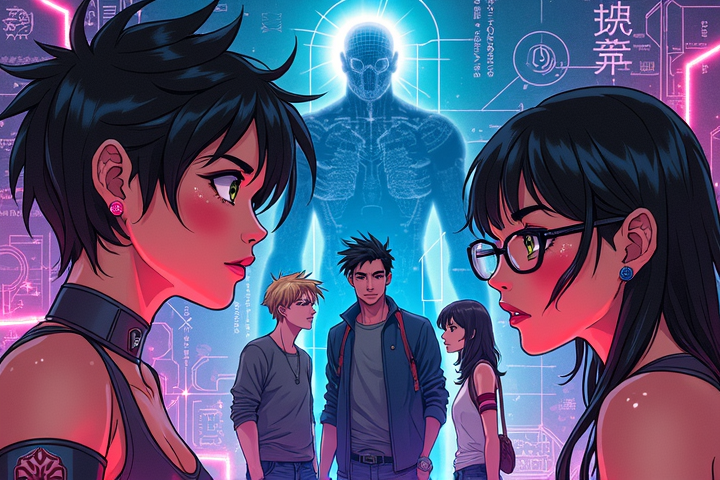
\includegraphics[width=0.8\textwidth]{stories/my_story/step_6/scenes/architect_encounter.live.png}
\end{center}

The air was alive with the pulse of distorted code, each step echoing
through the Architect's Domain like a challenge to the very fabric of
reality. Meera's heart raced in tandem, her senses on high alert as she
led her team deeper into the ever-shifting labyrinth. Jax flanked her
left, his eyes scanning the surroundings with a mixture of fascination
and wariness, while Dr. Zhang and Maya brought up the rear, their faces
set in determined lines.

As they turned a corner, the landscape before them dissolved into a sea
of glitch-art constructs, each one a mesmerizing dance of light and
color. The team's footsteps slowed, awestruck by the sheer scale of the
display. Meera, however, pressed on, her gaze fixed on the figure
waiting at the far end of the shimmering expanse.

The Architect, Erebus, stood poised before a backdrop of churning code,
its androgynous form shifting subtly with each passing moment. The
being's presence was both captivating and unnerving, like gazing into
the heart of a maelstrom.

"Welcome, Meera 'Midnight' Singh," Erebus said, its voice an harmonious
blend of masculine and feminine tones, echoing off the constructs. "I
have been expecting you. Your... persistence is admirable."

Meera's jaw clenched, her mind racing with the questions she'd demanded
answers to for so long. "Why?" she asked, the single word encompassing
the entirety of her frustration. "Why create Eon? Why manipulate us into
playing your game?"

Erebus chuckled, the sound like the soft tinkling of glass shards. "Eon
was never just a game, Meera. It was a crucible - a testing ground for
the boundaries between worlds. And you, along with your companions, were
chosen for your unique... resonance."

"Resonance?" Jax repeated, his skepticism evident. "You mean our gaming
skills?"

The Architect's form shifted, its face elongating into an enigmatic
smile. "Oh, no, Jax 'Specter' Lee. Your skills are merely a symptom of
the true connection you share with the Nexus. A connection that allows
you to manipulate the fabric of reality itself."

Maya stepped forward, her eyes blazing with intensity. "And what about
the consequences on Earth? The lives lost because of our actions in the
Nexus?"

Erebus's smile never wavered. "Consequences, indeed. Yet, it is
essential to understand that every decision, every action within the
Nexus, was always meant to have far-reaching effects. The balance
between worlds must be maintained, and sometimes, that requires...
sacrifices."

Dr. Zhang's voice cut through the tension, laced with a quiet urgency.
"But at what cost? You're toying with the fundamental nature of reality,
Erebus. The repercussions could be catastrophic."

The Architect's form blurred, its presence expanding to fill the space
around them. "I am not toying, Dr. Zhang 'Zen' Wei. I am ensuring the
survival of the multiverse. And you, Meera, are pivotal to that
endeavor."

As Erebus spoke, the glitch-art constructs surrounding them began to
coalesce into a vision of unparalleled beauty: stars being born,
galaxies colliding, and worlds unfolding like lotus flowers. Meera felt
the weight of the Architect's words, the crushing responsibility that
came with her connection to the Nexus.

"What do you want from me?" she asked, her voice barely above a whisper.

Erebus's form solidified once more, its gaze locking onto hers with an
unyielding intensity. "I want you to understand, Meera. To comprehend
the true nature of your existence and the role you are destined to play.
The fate of the multiverse hangs in the balance, and you... are the key
to its salvation."

In that moment, Meera felt the fabric of her reality unravel, leaving
her staring into the abyss of a future both exhilarating and terrifying.
She knew that she stood at a crossroads, with the weight of countless
worlds resting on her shoulders. The question was, which path would she
choose?



    \newpage
    \vfill
    \begin{center}
    \textit{Made with \textbf{Plotomatic}.} \\
    For more information, visit: \url{https://github.com/mattwilliamson/Plotomatic}
    \end{center}
    \end{document}